\chapter{Literature Study}
\label{chp:litreview}


\begin{figure}[htb!]
    \centering
    \input contents/chapt2/figs/literature_taxonomy_sections.tex
    \caption[A taxonomy of the autonomous racing literature with sections]{A taxonomy of the autonomous racing literature. The blue leaf nodes reference the section relevant to their description.}
    \label{fig:my_neuron}
\end{figure}

\section{Classic Pipeline}
\label{sec:classic}

\subsection{Trajectory planning}
\label{sec:trajectory_planning}

\begin{figure}[h]
    \centering
    \includegraphics{contents/chapt2/figs/classic_pipeline_planning.png}
    \caption{The classic autonomous driving pipeline with the trajectory planning modules relevant to this section colored in blue.}
    \label{fig:trajectory_planning}
\end{figure}

Global trajectory planning
geometric
\cite{Braghin2008} - shortest path vs minimum curvature

optimisation
\cite{Herrmann2019} - energy management
\cite{Herrmann2020} - optimization includes power usage of battery

genetic algorithms
\cite{Cardamone2010}
\cite{Vesel}

Local trajectory planning
\cite{Liniger2015a} - viability kernel for safe set of states
\cite{keefer2022} 
\cite{Wang2021}
\cite{Jeon2013} - a* shortest path search

\subsection{Control}
\label{sec:control}

most variations of MPC rely on tools from constrained optimization, which means that convexification (such as with quadratic approx- imation) of the cost function and first or second order approximations of the dynamics are required.
A more flexible MPC method is model predictive path
integral (MPPI) control, a sampling-based algorithm which can optimize for general cost criteria, convex or not. However, in prior work, MPPI could only be applied to systems with control affine dynamics.

\cite{Williams2017}
Relaxes the assumption that MPPI can only be applied to systems with linear dynamics.
Derive an update law to MPPI that is applicable to stochastic systems
by combining  model predictive control with model-based reinforcent learning.
This enables a purely data-driven approach to model learning in MPPI framework.
Vechile dynamics model is learned with MPPI 
Test controller  on a physical vehicle on a gravel track.
Vehicle performs well and is capable of performing aggressive driving manoeuvres on a gravel track. 

\begin{figure}[h]
    \centering
    \includegraphics{contents/chapt2/figs/classic_pipeline_control.png}
    \caption{The classic autonomous driving pipeline with the control modules relevant to this section colored in blue.}
    \label{fig:control}
\end{figure}

classic control

geometric control
latitude control
\cite{Coulter_1992} pure pursuit
\cite{Hoffmann2007} Stanley control

gg diagram
\cite{talvala2011} stabilise with lyapunov, use gg diagram

latitude and longitude control
\cite{Kritayakirana2010} gg diagram control


model predictive controllers

\cite{Pup2020} - characterising uncertainty in vehicle models from linearisation
\cite{Beal2013} - vehicle stabilisation at limits of handling
\cite{Liniger2019} - viability kernel to limit search space
\cite{Williams2016} - model predictive path integral control  
\cite{Hewing2018} - control cars under model inaccuracy with learning non-linear mpc

learning based control
\cite{Ji2018}
\cite{Brunner2018a}

\subsection{Full driving stacks}
\label{sec:full_driving_stacks}

\begin{figure}[h]
    \centering
    \includegraphics{contents/chapt2/figs/classic_pipeline_full_stack.png}
    \caption{The classic autonomous driving pipeline.}
    \label{fig:full_stack}
\end{figure}

\cite{Valls2018}
\cite{sherif2020}
\cite{Wischnewski2019} - kinematic state estimation
\cite{Vazquez2020} - in global planning
\cite{alvarez2022}

\section{End-to-end pipeline}
\label{sec:end_to_end}

The limitations of classical methods has led to research in learning-based systems that improve the vehicle dynamics model or action policy with real-world data and allow more complex cost formulations and non-linear dynamics \cite{Fuchs2021}.
Many learning approaches use an end-to-end pipeline, illustrated in Figure \ref{fig:end_to_end}, whereby a single neural network predicts control outputs from sensor data.
The neural networks used in end-to-end approaches are typically trained using imitation or reinforcement learning paradigms \cite{Betz2021}. We present a summary of research efforts into both approaches.

\begin{figure}[h]
    \centering
    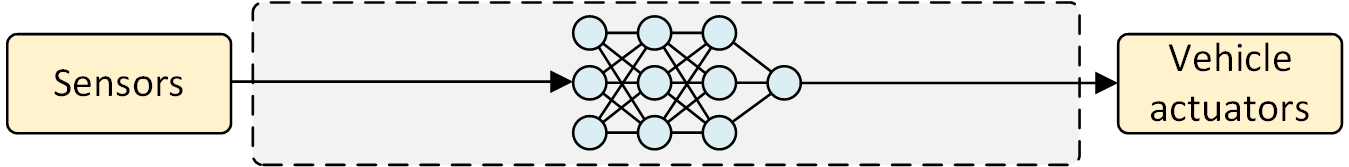
\includegraphics{contents/chapt2/figs/end_to_end_pipeline.png}
    \caption{The end-to-end autonomous driving pipeline.}
    \label{fig:end_to_end}
\end{figure}

\subsection{Imitation learning}
\label{sec:imitation_learning}

Imitation learning techniques train a neural network to mimic an expert such as a human or optimisation method.
The process is analogous to supervised learning, where labelled data is used to train an algorithm to predict outcomes on new data.
In the context of autonomous racing, the labelled training data is produced by allowing an optimisation method or human to interact with the vehicle.
This produces a set of control commands which act as the labels for the inputs to the neural network.
Supervised learning is then used to train an algorithm to predict control commands for new data \cite{Osa_2018}.

Imitation learning is the preferred method of training a neural network if it is feasible for an expert to demonstrate optimal behaviour but difficult to define a reward manually.
For instance, in some circumstances where vehicle manoeuvres are complex, correct driving behaviour may be more easily specified by a human demonstrator than manually designing a reward signal.
Furthermore, the expert limits the need for exploration, as required by reinforcement learning \cite{Osa_2018}.

A major benefit of imitation learning with neural networks is the cost of online computation: neural networks are far less computationally expensive to run than optimisation methods. This is demonstrated by Tatulea-Codrean et al. \cite{Tatulea-Codrean2020}, who train a neural network to mimic the policy of a non-linear MPC (NMPC). The NMPC is too computationally expensive for real-time control of the vehicle. 
However, the neural network computes the control command in a much faster time, enabling the deployment of the vehicle.

Imitation learning in conjunction with neural networks also have the benefit of being flexible towards their inputs. Whereas optimisation methods have strict requirements for the input as frequent state and boundary condition updates, imitation learning enables a neural network to learn from high dimensional inputs such as images from a video feed. This is accomplished by Mahmoud et al. \cite{Mahmoud2020} and Pan et al. \cite{Pan2017a}. 
Pan et al. \cite{Pan2017a} showcase the usefulness of this property by using imitation learning to relax hardware requirements and reduce the cost of the vehicle sensor suit. 
Their neural network is trained to mimic an MPC on a vehicle with two sensor suits: an IMU and GPS unit worth 6000\$, and 500\$ camera.
While the MPC requires the 6000\$ IMU and GPS, the neural network is trained to execute the same policy on the 500\$ camera.

The flexibility of neural networks towards their inputs is related to another useful property: robustness to sensor noise and failure. 
This property is showcased well by Lee et al. \cite{Lee2019}, who use imitation learning to create an ensemble of bayesian neural networks (BNN) on different sensor inputs to create a redundant control policy. 
The algorithm is robust to sensor noise and even multiple sensor failures, which was not possible using more traditional optimisation methods.

From these examples we see that imitation learning learning with neural networks is a powerful tool.
However, Wadekar et al. \cite{Wadekar2021} highlight some weaknesses of the imitation learning technique.
The neural network policy will not match the expert policy exactly. 
Since policy affects the distribution of states that the vehicle encounters, the vehicle may encounter a scenario for which no expert training data was generated during training, in which case it is likely to take an incorrect action \cite{Osa_2018}.
Furthermore, Wadekar et al. \cite{Wadekar2021} describe that the data collected by the expert must be curated so that the agent does not learn any undesirable behaviour.
Perhaps the most undesirable characteristic of imitation learning is that it requires expert training data.
This makes it unsuitable for scenarios where expert training data is not available, as in cases where optimisation methods fail \cite{Fuchs2021a}.
As such, we turn towards a method for training neural networks for control tasks that does not require expert training data.

\subsection{Reinforcement learning}
\label{sec:reinforcement_learning}

Reinforcement learning optimises a neural network policy to maximise a scalar reward signal through direct interaction with the environment \cite{Plaat_2022}. 
The benefits of using reinforcement learning are the same as the imitation learning approach, i.e., less stringent sensor requirements, robustness to sensor failure, and fast online execution time. However, the technique allows for more complex cost formulation than what is possible with even state of the art expert optimisation methods and negates the need for expert training data \cite{Fuchs2021}.
%Reinforcement learning approaches may be categorized according to their action selection method. Whereas model-based methods use a model of the vehicle and environment to plan ahead, model-free methods select an action based only on past experience. 


Several research efforts into reinforcement learning applied to autonomous racing have been aimed at creating pixel to control algorithms. 
Perot et al. \cite{Perot2017} and Jaritz et al. \cite{Jaritz2018} are early works in model-free reinforcement learning applied to autonomous racing that present such pixel to control algorithms for racing in the video game World Rally Cross 6.
Both approaches utilise a convolutional neural network (CNN) with long short-term memeory (LSTM). 
Jaritz et al. \cite{Jaritz2018} state that a score given at the end of the race is too sparse for the agent to learn effectively.
They therefore introduce a continuous reward schema.
Continuous reward schemas have been used by every approach reviewed since Perot et al. \cite{Perot2017} and Jaritz et al. \cite{Jaritz2018}.
However, the approaches show that pixel to control is both extremely inefficient, as both Jaritz et al. \cite{Jaritz2018} and Perot et al. \cite{Perot2017} train their agent for 80 million steps.



Another pixel to control strategy is developed by Schwarting et al. \cite{Schwarting2021}, who apply model-based reinforcement learning to openAI gym's two player racecar environment.
When multiple vehicles are involved, the opponents behaviour must be taken into account.
However, these behavioral and environmental features may be too complex to be captured by MPC or purely game-theoretic approaches that assume perfect knowledge of the state of all vehicles.
Schwarting et al. \cite{Schwarting2021} showcase the strength of reinforcement learning to generate policies without perfect knowledge of the environment.
Their solution learns a model of the world (including the opponent behaviour) using a neural network.
This model is then used to generate imagined gameplay experiences to train the agent on.


A more recent and state of the art approach is presented by Fuchs et al. \cite{Fuchs2021}, who creates a model-free soft actor-critic (SAC) agent that achieves lap times on par with competitive e-sports drivers in the racing game Gran Turismo Sport.
Key to their approach is careful selection of hand-crafted input features that include: 1) the vehicles velocity $\pmb{v}_t \in \mathbb{R}^3$, 2) acceleration $\pmb{\dot{v}}_t \in \mathbb{R}^3$, 3) distance measurements of $M$ rangefinders $\pmb{d}_t \in \mathbb{R}^M$, 4) the previous steering command $\delta_{t-1}$, 5) a binary flag indicating wall contact, and 6) $N$ sampled curvature measurements of the track centerline $\pmb{c}_t \in \mathbb{R}^N$.
These are important input features, as most other reinforcement learning approaches that do not utilise a pixel to control strategy use a selection of these features as input to their neural network.
Fuchs et al. \cite{Fuchs2021} also introduce a continuous progress term into the reward signal, while penalising the agent for making contact with the track boundary:
\begin{equation}
    r_t = r_{t}^{\text{progress}} - 
    \begin{cases}
    c_w \| \pmb{v}_t \| & \text{if in contact with wall} \\
    0 & \text{otherwise}
    \end{cases}
\end{equation}
where $c_w$ is a tuned constant.
Although their implementation remains in simulation, Fuchs et al. \cite{Fuchs2021} do measure the effect of vehicle model inaccuracies by changing the parameters of the vehicle model between training and testing. They find that increased tire friction causes the agent to steer more aggressively leading to brief contact with the inside wall. A decrease in tire friction causes the agent to take corners slightly wide resulting in contact with the outside.
They also measure the effect of delays to the agents inference, finding that delays of greater than 100ms leads to track boundary contact. 
However, it is not clear from Fuchs et al. \cite{Fuchs2021} what degree of model inaccuracy results in collisions.


Song et al. \cite{Song2021} extends the work from Fuchs et al. \cite{Fuchs2021} to a multi-agent setting, training an agent to overtake other vehicles in Gran Turismo Sport.
key to their success is the use of curriculum learning, whereby the agent is trained to solve increasingly difficult tasks by adding components to both the environment and reward signal. 
The agent is trained to race on its own before another vehicle is added to the simulation, and the reward signal is modified to encourage the agent to make progress relative to the other vehicle.
This showcases the strength of reinforcement learning over optimisation methods: while optimisation algorithms rely on the convexification of cost functions, reinforcement learning agents can learn to solve difficult tasks from complex cost functions.


We now move away from now games and discuss research efforts that more directly address the sim2real gap and deployment onto physical cars.
Niu et al. \cite{Niu2020} anticipate that the reinforcement learning algorithm may select an unsafe action.
To prevent this, they propose a model-based safety controller that acts as a safeguard mechanism to prevent the agent from selecting unsafe actions.
Furthermore, they foresee that the safety module's reliance on an accurate vehicle model presents an issue. 
As such, a neural network is used to learn a vehicle model online that eventually replaces the initial assumed vehicle model.
This idea of improving a vehicle model after the vehicle is deployed is a commonplace sim2real practice.
Another benefit of the safety controller is that it constricts the agent's exploration, allowing the policy to converge faster and more robustly.


Another issue that presents itself during physical deployment is that of control smoothness. 
Sudden control actions will induce excessive mechanical wear and cause the vehicle to exhibit dangerous behaviour.
Hsu et al. \cite{hsu2022} identify this issue andapply Conditioning for Action Policy Smoothness (CAPS) to smooth the control action of the vehicle.
Although Hsu et al. \cite{hsu2022} do not directly address model inaccuracies, their policy smoothing approach produces a conservative policy which is expected to increase performance and safety in settings where the model inaccuracies occur.
This is because a smoother policy results in less lateral and longitudinal acceleration and does not bring the vehicle as close to its handling limits as a jerkier policy.


More sim2real practices are explored by Chisari et al. \cite{Chisari2021}, who deploy a soft actor-critic model-free reinforcement learning algorithm onto a physical vehicle.
They make the agent policy robust to real-world transfer training in simulation with a slightly randomised vehicle model.
The agent policy is then refined by retraining the neural network after the physical vehicle is deployed.
This allows the reinforcement learning algorithms to achieve lap times but have the number of track boundary collisions as an MPC controller.
Ivanov et al. \cite{Ivanov2020} take a similar approach to Chisari et al. \cite{Chisari2021} by training an agent with model randomisation, but are not able to achieve robustness to the sim2real transfer.

The final end-to-end approach we discuss is by Brunbauer et al. \cite{brunnbauer}, who demonstrate demonstrate the effectiveness of advanced model- based deep RL compared to model-free agents in the real-world application of autonomous racing.
Brunnbauer et al. \cite{brunnbauer} deploy the model-based Dreamer reinforcement learning algorithm by Hafner et al. \cite{Hafner2019a} on a physical F1tenth vehicle.
Their algorithm learns an observation model which is used to predict agent-environemnt interactions.
It then learns a policy purely on imagined sequences using the observation model, without interaction with the environment.
This results in safe and data-efficient learning.

\begin{landscape}
    \newcolumntype{a}{>{\hsize=1\hsize \centering\arraybackslash}X}
\newcolumntype{d}{>{\hsize=.5\hsize \centering\arraybackslash}X}
\newcolumntype{e}{>{\hsize=2\hsize \centering\arraybackslash}X}


\begin{table}[h]
\centering
\begin{tabularx}{21cm}{|a|d|d|d|d|e|}
    
    \hline
    \small \textbf{Name} & \small \textbf{Model-based} & \small \textbf{Multi-agent} & \small \textbf{Input} & \small \textbf{Physical vehicle} & \small \textbf{sim2real approach} \\
    \hline
    \small Schwarting et al. \cite{Schwarting2021} & \checkmark & \checkmark & \small game image & & - \\
    \hline
    \small Brunnbauer et al. \cite{brunnbauer2021} & \checkmark & & \small features & \checkmark & - \\
    \hline
    \small Perot et al. \cite{Perot2017} & & & \small game image & & - \\
    \hline
    \small Jaritz et al.  \cite{Jaritz2018} & & & \small game image & & - \\
    \hline 
    \small Fuchs et al. \cite{Fuchs2021} & & & \small features & & \small Test effects of model inaccuracy in simulation \\
    \hline
    \small Remonda et al. \cite{Remonda2021} & & & \small features & \checkmark & - \\
    \hline 
    \small Song et al. \cite{Song2021} & & \checkmark & \small features & & - \\
    \hline
    \small Niu et al. \cite{Niu2020} & & & \small features & & \small Safety module based on learned vehicle model prevents agent from selecting unsafe actions. \\
    \hline
    \small Chisari et al. \cite{Chisari2021} & & & \small features & \checkmark & \small Parameter randomisation while training, policy refinement after deployment \\
    \hline
    \small Ivanov et al. \cite{Ivanov2020} & & & \small features & \checkmark & \small Parameter randomisation while training \\
    \hline
    \small Hsu et al. \cite{hsu2022} & & & \small image & \checkmark & \small Control action smoothing \\
    \hline

\end{tabularx}
\caption[A summary of end-to-end reinforcement learning approaches for autonomous racing]{A summary of end-to-end reinforcement learning approaches for autonomous racing.}
\label{table:autonomous_racing_rl_summary}
\end{table} 

    \footnote{The absence of a tick in the model-based, multi-agent , and physical vehicle columns indicate that the approach was model-free, single-agent and simulation only, respectively. \label{footnote_1}}
\end{landscape}



\section{Partial end-to-end pipeline}
\label{sec:partial_end_to_end}

Wrapping the entirety of a perception-planning-control
pipeline into one black-box network can exacerbate the the problem of overfitting, as a single deep network needs to learn all three high-level tasks as part of a single model. We show in our experiments in section 6 that just because an end-to-end (pixels to control) method performs well on unseen validation data (as measured Root-Mean-Squared error), that does not mean that same method contains a useful driving strategy that will perform well in an actual live-driving test \cite{Weiss2020a}.

\begin{figure}[h]
    \centering
    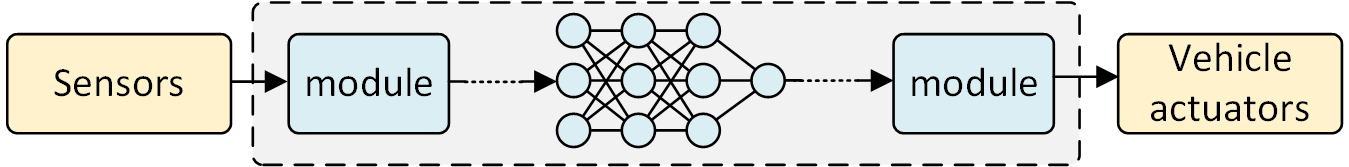
\includegraphics{contents/chapt2/figs/partial_end_to_end_pipeline.png}
    \caption{The partial end-to-end autonomous driving pipeline.}
    \label{fig:partial_end_to_end}
\end{figure}

Reinforcement learning
\cite{Evans2021b} - learning local planning
Evans integrates a path follower reinforcement learning agent
the reinforcement learning agent modifies the reference steering angle of the path follower that follows a global plan
The goal is to learn obstacle avoidance.
The agent is required to navigate in an environment with obstacles placed randomly in unknown locations.
Evans measures similar performance for both the end-to-end and partial-end-to-end method.


\cite{Ghignone2022} - rl for following trajectory. Outperforms mpc
exploiting the heuristic nature of RL while leveraging the reliability of traditional planning methods in a hierarchical control structure.
trains agent under varying tire conditions to generalise to different model parameters
Outperforms MPC with 2.7 times lower crash ratio in model mismatch setting
and computes 40 times faster than the MPC.
6.7 times lower crash ratio than end-to-end learning under model mismatch.
Propose solution tracks a spatial trajectory generated by a high level planner
Observation includes a sample of the path ahead of the agent




Neural network local planner
\cite{Weiss2020a} - local planning
Weiss et al. \cite{Weiss2020a} use a neural network trained with imitation learning as a local planner.
The neural network maps is given a sequence of game images and outputs a path.
Weiss et al. \cite{Weiss2020a} take an idea from classical global planning: parameterising the path as a function.
In this case, the path is described as a Bezier curve. 
The neural network outputs the parameters for this bezier curve that describe the $x$ and $y$ coordinates as a function of time.
The velocity is the time derivative of the bezier curve.
The path formed by the bezier curve is followed by a pure pursuit path tracker.
Bang-bang control is used for the velocity: maximum acceleration and deceleration is applied when the current velocity is lower than and higher than desired, respectively.
Weiss et al. \cite{Weiss2020a} reports that their approach outperforms the end-to-end baseline by a large margin. 

\cite{Capo2020} - short term trajectory planning using rl.
neural network predicts a point on the track ahead of the car.
the point is steered towards using low level control logic.
The approach outperformed end-to-end approaches in terms of distance races and generalisation across different tracks.
Does not take into account model uncertainty.


All partial end-to-end pipeline results indicate that the partial end-to-end pipeline outperforms the end-to-end pipeline.


\begin{table}[h]
\centering
\begin{tabularx}{\textwidth}{|b{1.6cm}|X|X|X|b{4cm}|}
    \hline
    \textbf{Name} & \textbf{Learning method} & \textbf{Learned trajectory planner} & \textbf{Learned controller} & \textbf{sim2real approach} \\
    \hline
    Weiss et al. \cite{Weiss2020a} & IL & \checkmark & & - \\
    \hline
    Capo et al. \cite{Capo2020} & RL & \checkmark & & - \\
    \hline
    Evans et al. \cite{Evans2021b} & RL &  & \checkmark & - \\
    \hline
    Ghignone et al. \cite{Ghignone2022} & RL &  & \checkmark & Randomise vehicle model parameters while training \\
    \hline
\end{tabularx}
\caption[A summary of partial end-to-end approaches for autonomous racing]{A summary of partial end-to-end approaches for autonomous racing}
\label{table:autonomous_racing_partial_end_to_end_summary}
\end{table} 



\section{Summary}

\begin{figure}
    \centering
    \input contents/chapt2/figs/literature_taxonomy_articles.tex
    \caption[A taxonomy of the autonomous racing literature with articles]{A taxonomy of the autonomous racing. The blue leaf nodes reference the articles relevant to their description.}
    \label{fig:literature_taxonomy_1}
\end{figure}
